
\begin{figure*}[t]
    \begin{center}
    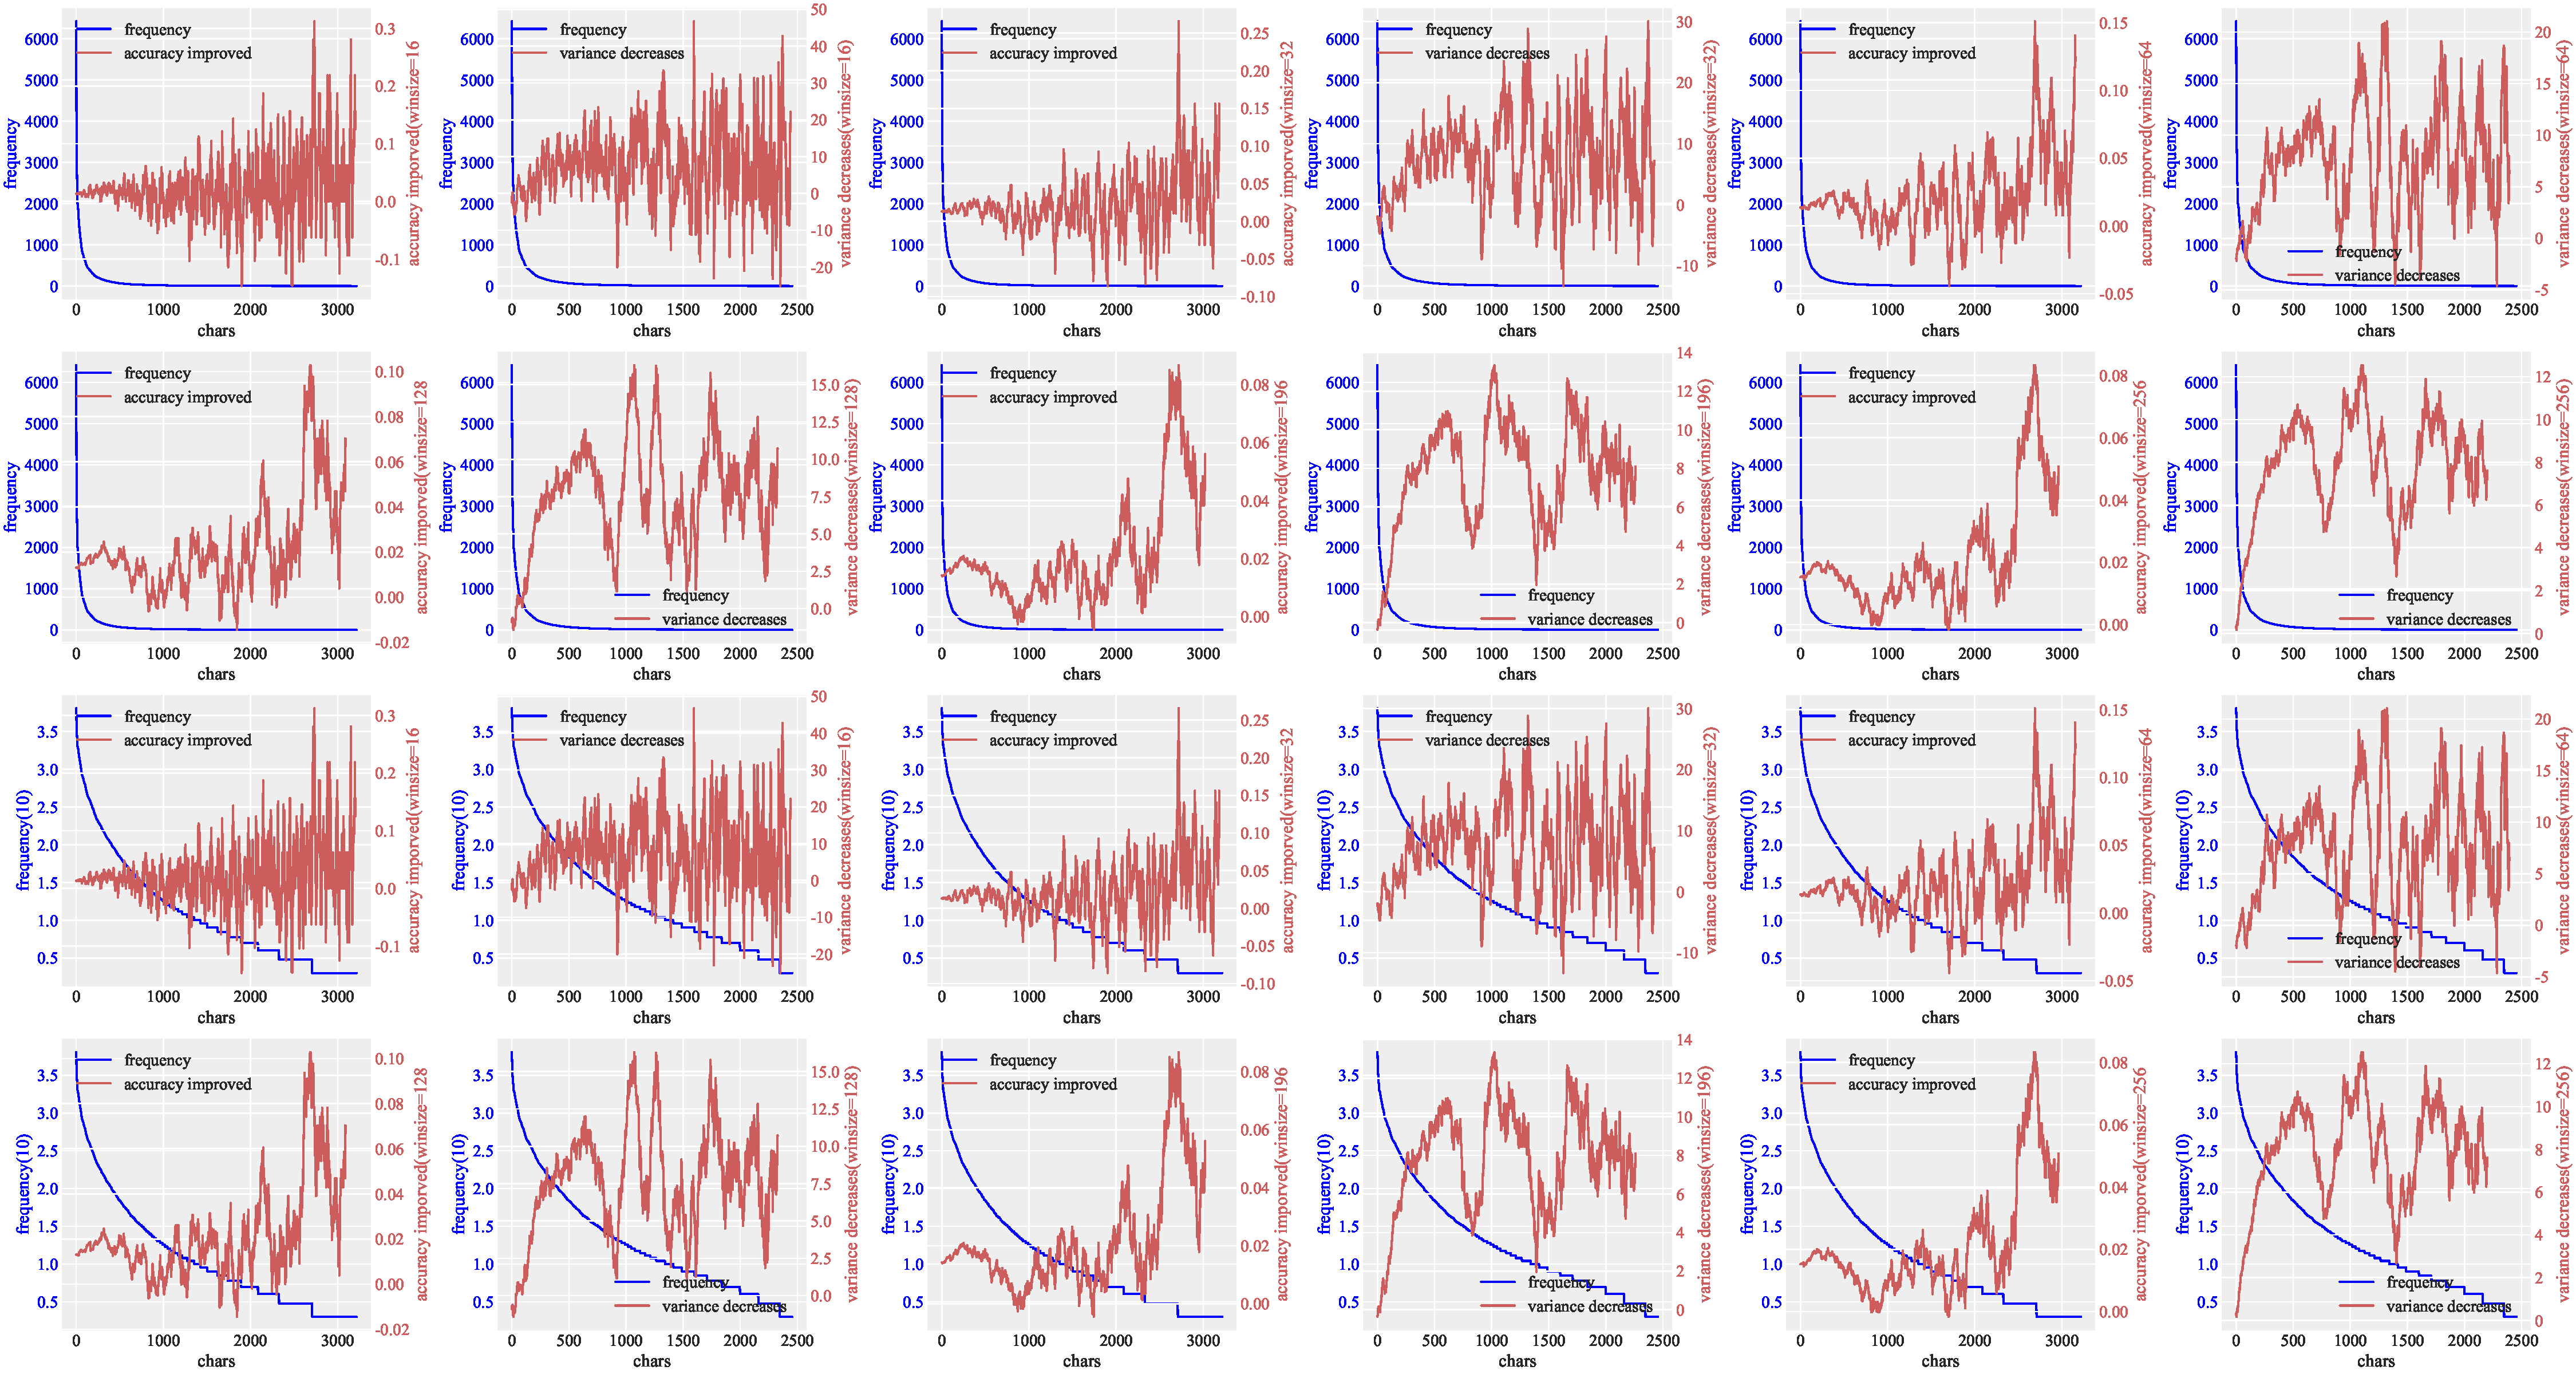
\includegraphics[width=1.0\linewidth]{figures/freqvsimprovement.pdf}
    \end{center}
    \caption{Frequency and accuracy imporved. In order to more effectively validate the relationship between frequency and performance, we employed different logarithmic bases for character frequency and applied various smoothing factors to accuracy to visualize the overall results. It is evident that the improvement in tail performance is significantly greater than that in the head.}
    \label{fig:freqvsimprovement}
\end{figure*}

    